\chapter[Analise dos Resultados]{Análise dos Resultados e Discussões}
\addcontentsline{toc}{chapter}{analise dos Resultados e discussões}
\label{chap:analiseResultados}

Este capítulo apresenta a análise dos resultados obtidos com a execução dos modelos de treinamento centralizado e distribuído. Além disso, é exposta a análise do autor referente aos dados coletados e as impressões obtidas durante a execução dos experimentos. Inicialmente há a apresentação dos resultados obtidos, acompanhada pela \hyperref{sec:resultados}{Análise dos Resultados}. Posteriormente, são discutidas as dificuldades e limitações encontradas durante a execução dos experimentos.

Serão apresentados e discutidos os desempenhos dos modelos desenvolvidos ao longo do projeto, tanto no contexto centralizado quanto no federado. Três modelos centralizados foram implementados: uma rede neural convolucional (CNN), uma rede neural multicamadas (MLP) e uma rede neural profunda (DNN). Esses modelos serão comparados com o modelo de aprendizado federado, permitindo uma análise detalhada das métricas obtidas, como acurácia, precisão, sensibilidade, F1-score e o tempo de processamento. A comparação entre os modelos visa identificar as vantagens e limitações de cada abordagem, destacando o impacto do aprendizado federado na preservação de privacidade dos dados e na eficiência do treinamento distribuído.

\section{Análise dos Resultados}
\label{sec:resultados}

\section{Desempenho dos Modelos Centralizados}

\subsection{Modelo Centralizado - Rede neural convolucional}

Um dos modelos centralizados foi implementado utilizando uma rede neural convolucional (CNN) e treinado sobre o conjunto de dados Fashion-MNIST. O modelo foi desenhado com duas camadas convolucionais seguidas de camadas de pooling, aplicando a técnica de dropout para evitar o overfitting. O modelo foi treinado com 50 épocas, utilizando a otimização Adam, com uma taxa de aprendizado ajustada para 0,001 para garantir um aprendizado gradual. O objetivo foi avaliar o desempenho de um modelo CNN simples, mas com regularização, em um conjunto de dados com complexidade visual moderada, como o Fashion-MNIST.

\begin{figure}[ht]
    \centering
    \caption{Curvas de acurácia do modelo centralizado - CNN}
    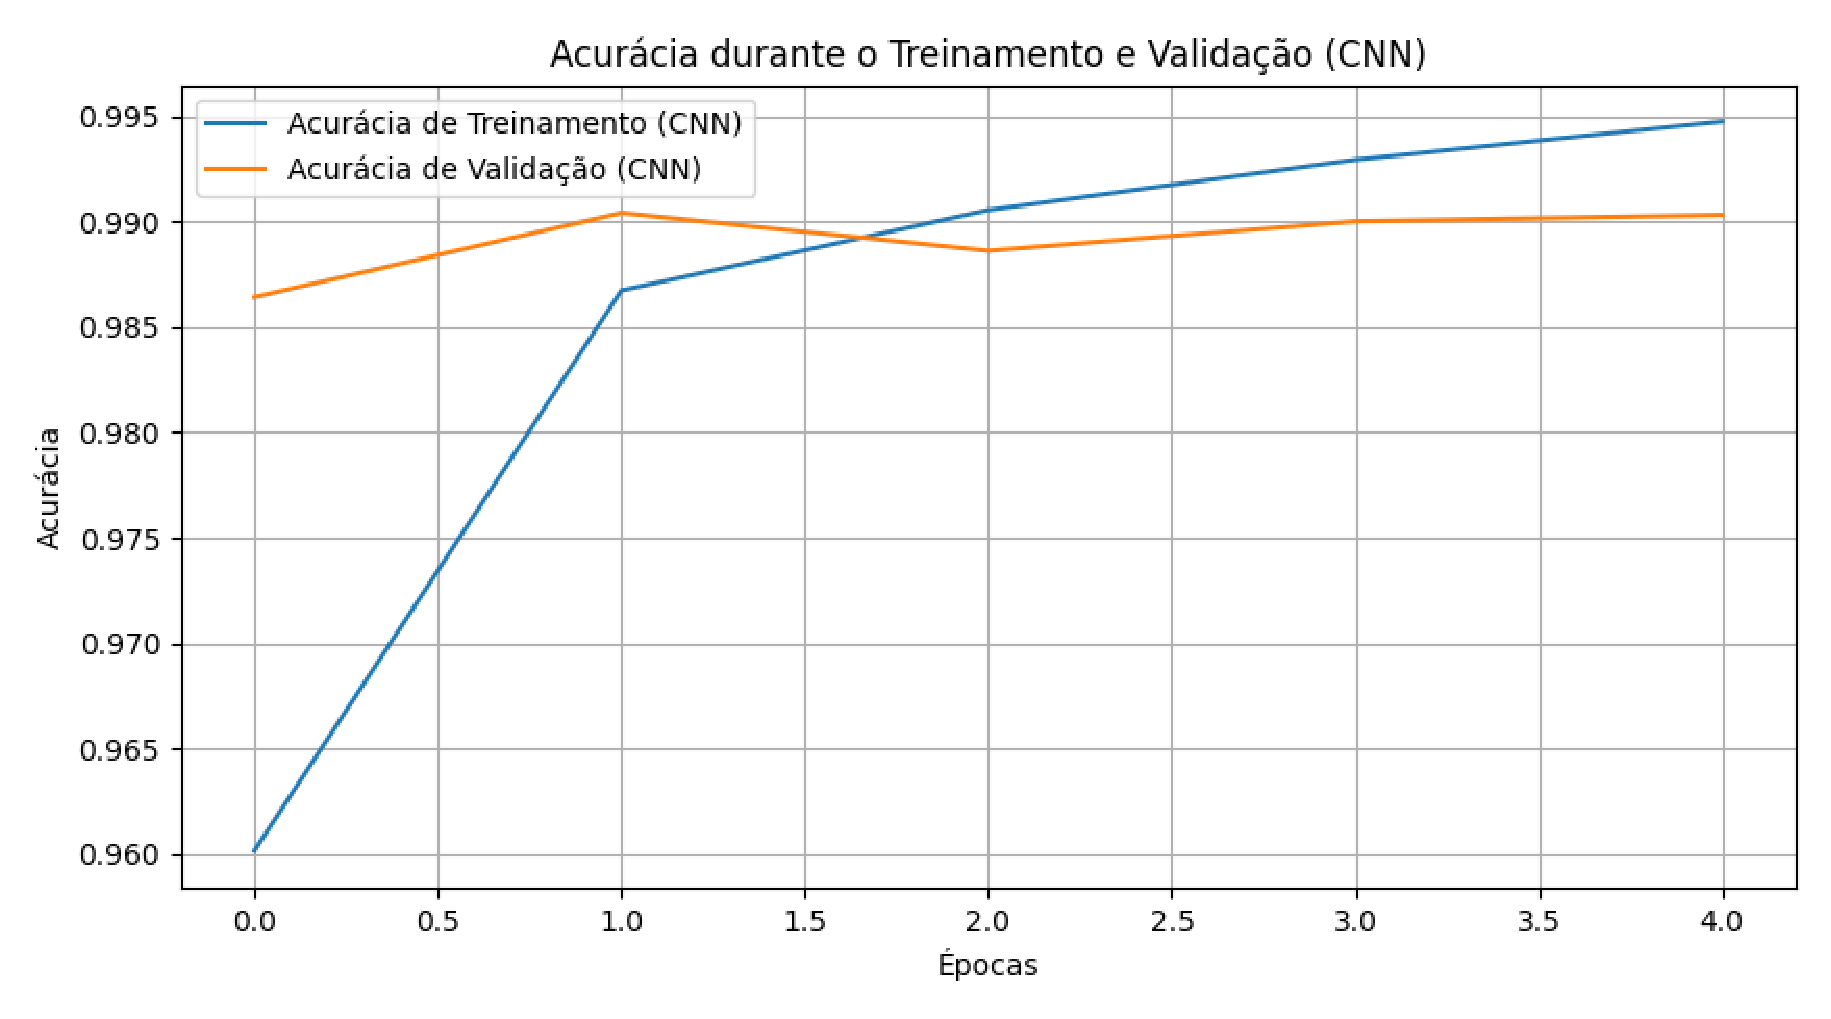
\includegraphics[scale=0.4]{figuras/analiseResultados/acuracyCNN.eps}
    \label{fig:acuracyCNN}
    \fonte{Elaborado pelo autor.}
\end{figure}

Durante o treinamento, como observado na Figura \ref{fig:acuracyCNN}, o modelo apresentou uma curva de aprendizado consistente, com acurácia de treino subindo de 72,57\% na primeira época para cerca de 96,71\% na última época. Já nos dados de teste, a acurácia se estabilizou em torno de 91,40\%. Esses resultados mostram que o modelo CNN consegue generalizar bem para os dados de teste, sem apresentar sinais claros de overfitting, apesar de ter utilizado dropout para regularização. Isso é evidenciado também pelo comportamento da perda, que foi reduzida de 0,7628 na primeira época para 0,0811 na última.

\begin{figure}[ht]
    \centering
    \caption{Curvas de perda do modelo centralizado - CNN}
    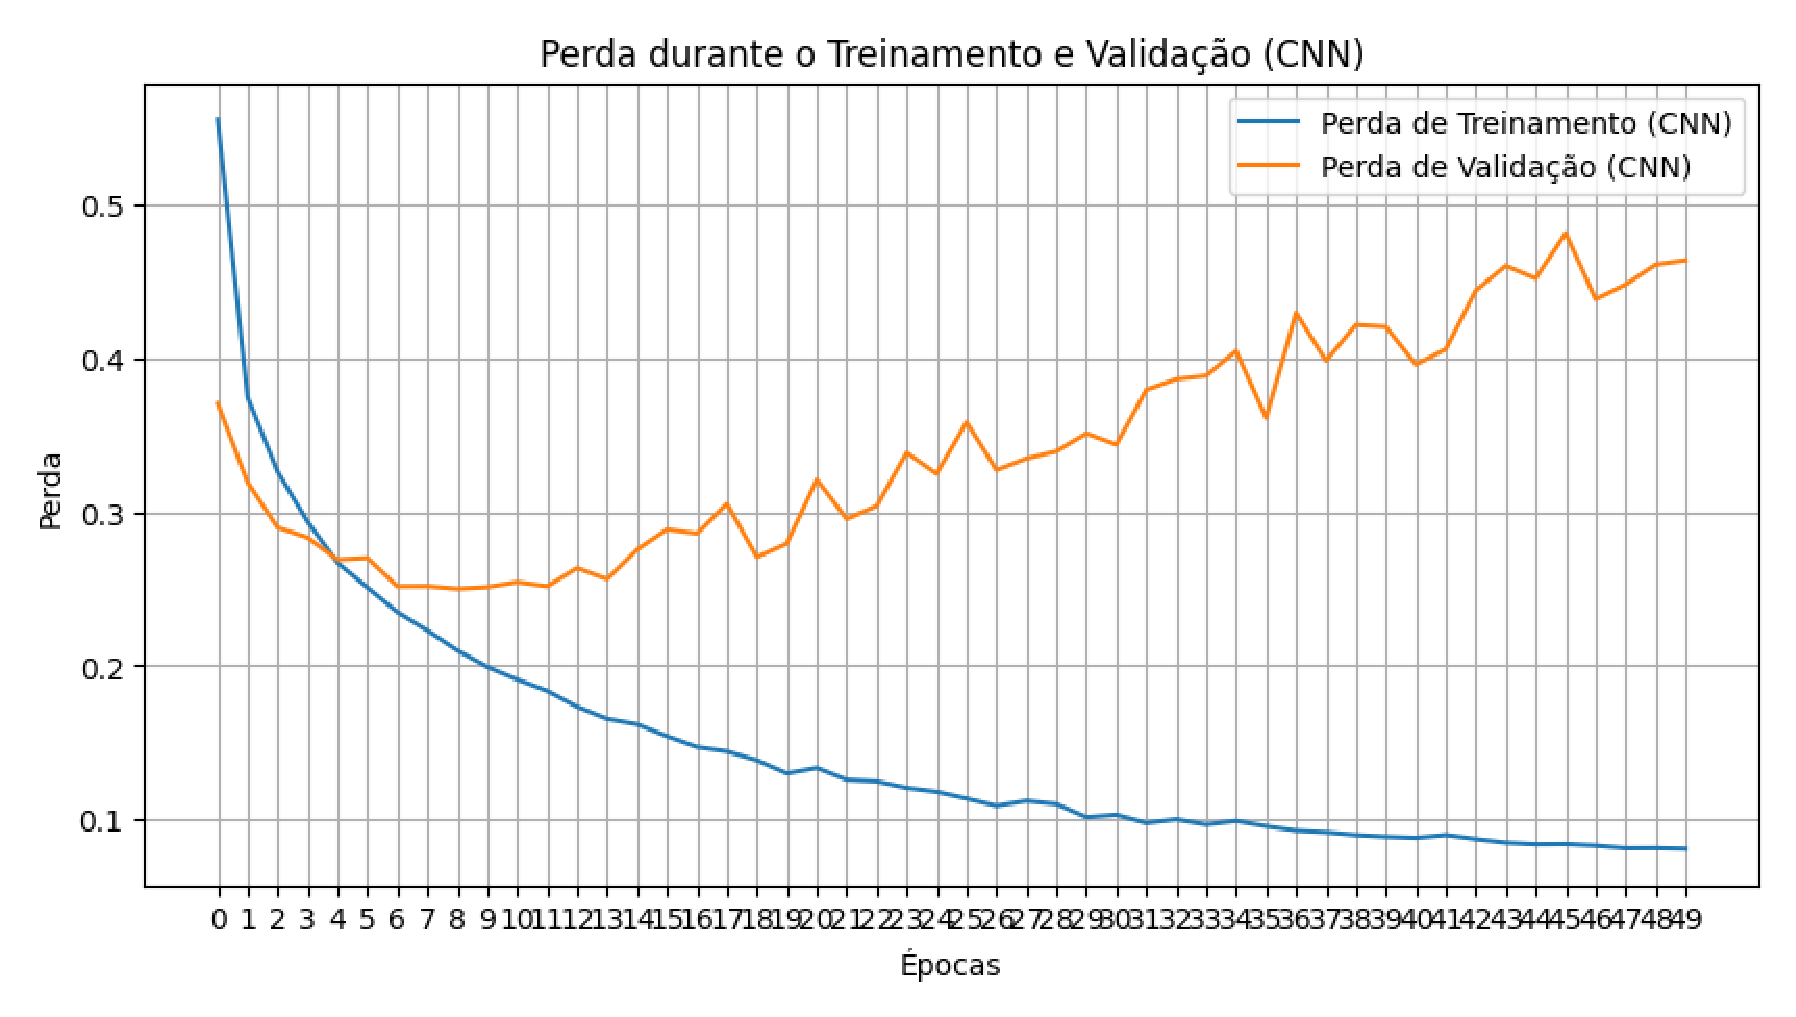
\includegraphics[scale=0.4]{figuras/analiseResultados/lossCNN.eps}
    \label{fig:lossCNN}
    \fonte{Elaborado pelo autor.}
\end{figure}

A análise das métricas de validação mostra que o modelo atingiu 91,33\% de acurácia nos dados de teste (\ref{fig:lossCNN}). A perda de validação, embora tenha flutuado ao longo das épocas, manteve-se em níveis aceitáveis, finalizando em 0,4632. A validação revelou que o modelo manteve uma consistência de generalização ao longo do treinamento, mas a perda levemente elevada no final das épocas indica que ainda há espaço para melhorias na otimização do modelo, ou ajustes adicionais para regularização mais eficiente.

Em termos de tempo de treinamento, o modelo foi treinado por aproximadamente 3816 segundos (cerca de 63 minutos), o que reflete a complexidade do modelo CNN em comparação com arquiteturas mais simples como MLP. Apesar desse tempo considerável, os resultados sugerem que o esforço computacional é justificado pelo ganho de desempenho, especialmente na tarefa de classificação de imagens mais complexas, como as da base Fashion-MNIST. Comparando com o modelo federado, a principal vantagem aqui está no tempo de treinamento, uma vez que a centralização dos dados acelera significativamente o processo, eliminando a latência e a complexidade da comunicação entre dispositivos, que são características do aprendizado federado.

\subsection{Modelo Centralizado - Rede neural multicamadas}

O modelo MLP foi construído com uma arquitetura composta por camadas densas totalmente conectadas, com três camadas ocultas contendo 512, 256 e 128 neurônios, respectivamente. Além disso, foi implementado um mecanismo de regularização através de dropout, que visa reduzir o overfitting ao desativar uma fração de neurônios durante o treinamento. A função de ativação utilizada foi a ReLU, com a camada final sendo uma softmax, apropriada para classificação multiclasse.

Durante o treinamento, que ocorreu ao longo de 50 épocas, o modelo mostrou uma melhoria gradual em termos de acurácia, partindo de 73,37\% na primeira época e atingindo 91,02\% ao final. A precisão nos dados de teste alcançou 89,09\%, o que reflete a capacidade do modelo de generalizar razoavelmente bem para dados não vistos (\ref{fig:acuracyMLP}). A perda de validação oscilou ao longo do processo de treinamento, com uma ligeira tendência de queda, indicando que o modelo estava efetivamente aprendendo, embora a diferença entre perda de treinamento e perda de validação sugira que um ajuste fino adicional poderia melhorar ainda mais o desempenho.

\begin{figure}[ht]
    \centering
    \caption{Curvas de acurácia do modelo centralizado - MLP}
    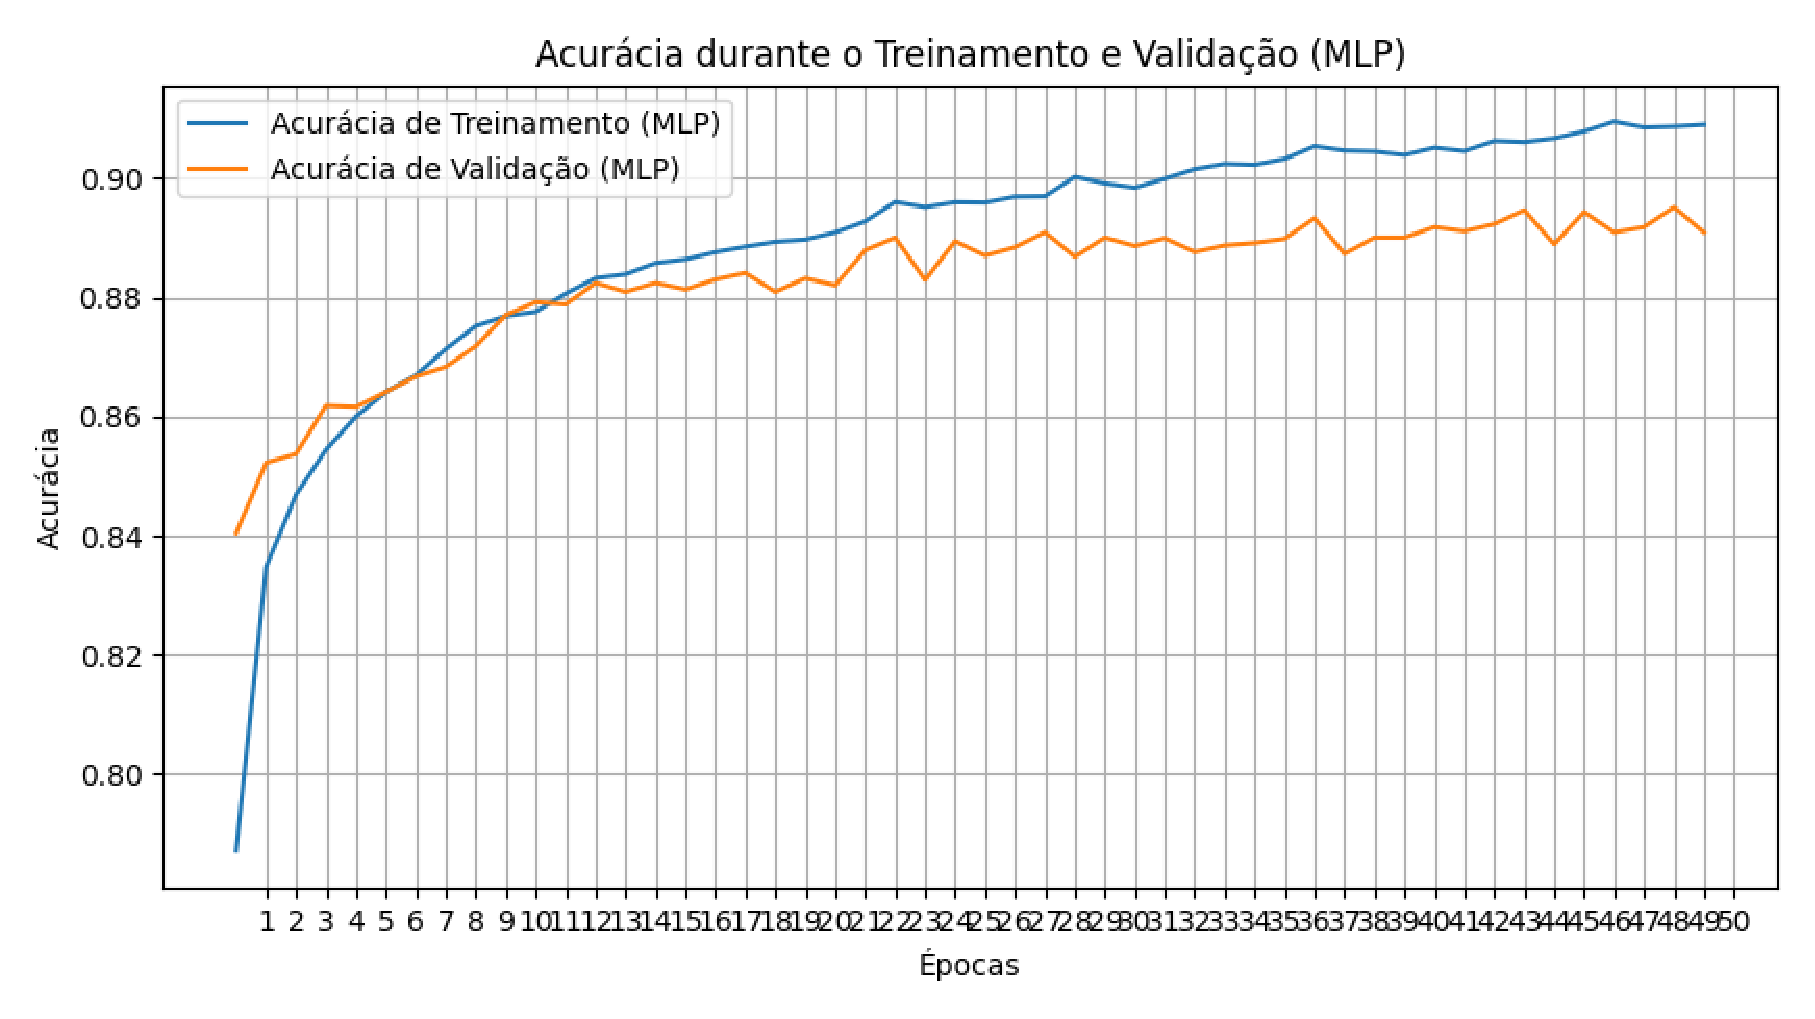
\includegraphics[scale=0.4]{figuras/analiseResultados/acuracyMLP.eps}
    \label{fig:acuracyMLP}
    \fonte{Elaborado pelo autor.}
\end{figure}

Analisando as métricas obtidas, a acurácia se estabilizou em torno de 89\% nos dados de teste, sugerindo que o MLP foi capaz de capturar padrões relevantes para a tarefa de classificação de imagens da base de dados Fashion-MNIST. A regularização por dropout também desempenhou um papel fundamental na mitigação do overfitting, permitindo que o modelo mantivesse um bom desempenho ao lidar com dados de teste. No entanto, em comparação com outros modelos como a CNN, o MLP mostra-se ligeiramente inferior, especialmente em termos de generalização para novas amostras, o que é esperado, dado que a CNN é mais eficaz para capturar padrões espaciais em dados de imagem.

\begin{figure}[ht]
    \centering
    \caption{Curvas de perda do modelo centralizado - MLP}
    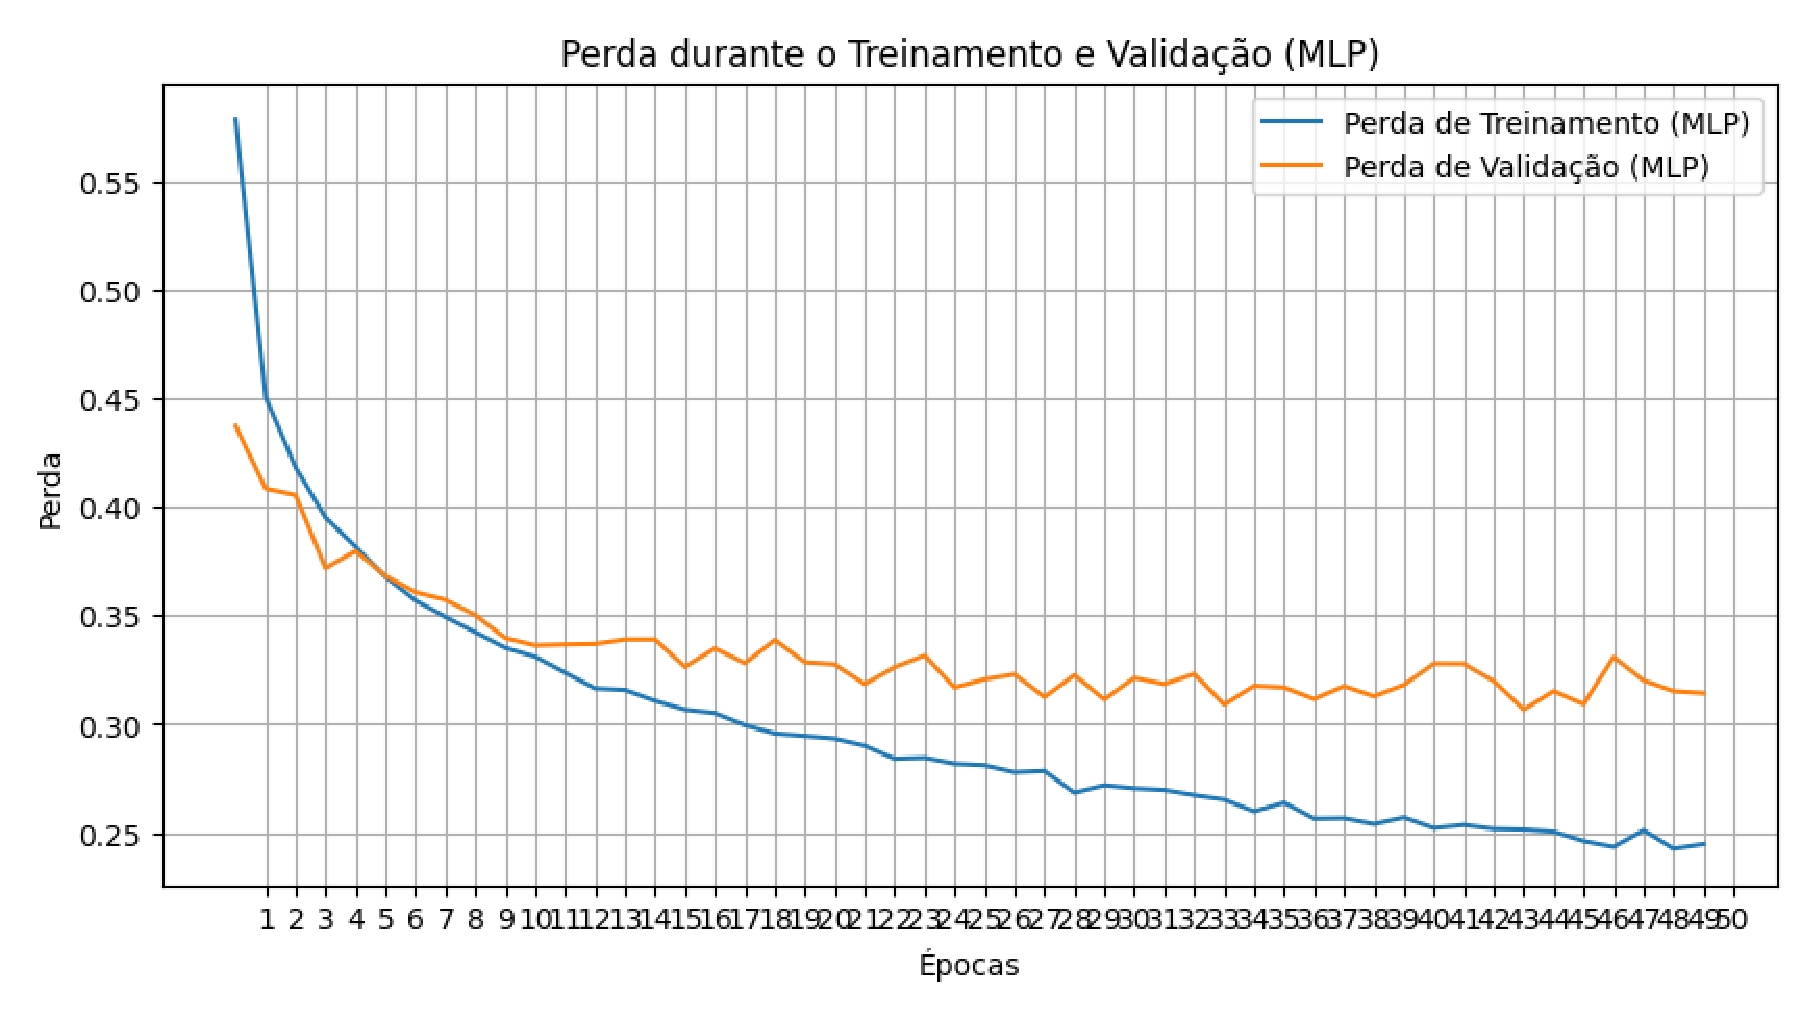
\includegraphics[scale=0.4]{figuras/analiseResultados/lossMLP.eps}
    \label{fig:lossMLP}
    \fonte{Elaborado pelo autor.}
\end{figure}

Em termos de tempo de treinamento, o MLP foi significativamente mais rápido do que a CNN, completando o treinamento em aproximadamente 22 minutos (1348 segundos). Embora esse modelo tenha se mostrado eficiente em termos de tempo, a compensação foi uma precisão ligeiramente inferior e uma maior suscetibilidade ao overfitting. Isso reflete uma característica comum dos MLPs em comparação com arquiteturas mais complexas, como as CNNs, que conseguem captar melhor as relações espaciais intrínsecas aos dados de imagem.

\subsection{Modelo Centralizado - Rede neural profunda}

O modelo foi composto por uma camada de entrada que recebe as imagens de 28x28, que são achatadas para vetores, seguida por múltiplas camadas densas, começando com 1024 neurônios, reduzindo gradativamente para 512, 256 e 128 neurônios. Além disso, foi implementada uma técnica de dropout de 50\% após a primeira camada densa, visando reduzir o overfitting. As camadas ocultas utilizam a função de ativação ReLU e a camada final utiliza softmax, apropriada para classificação multiclasse.

\begin{figure}[ht]
    \centering
    \caption{Curvas de acurácia do modelo centralizado - DNN}
    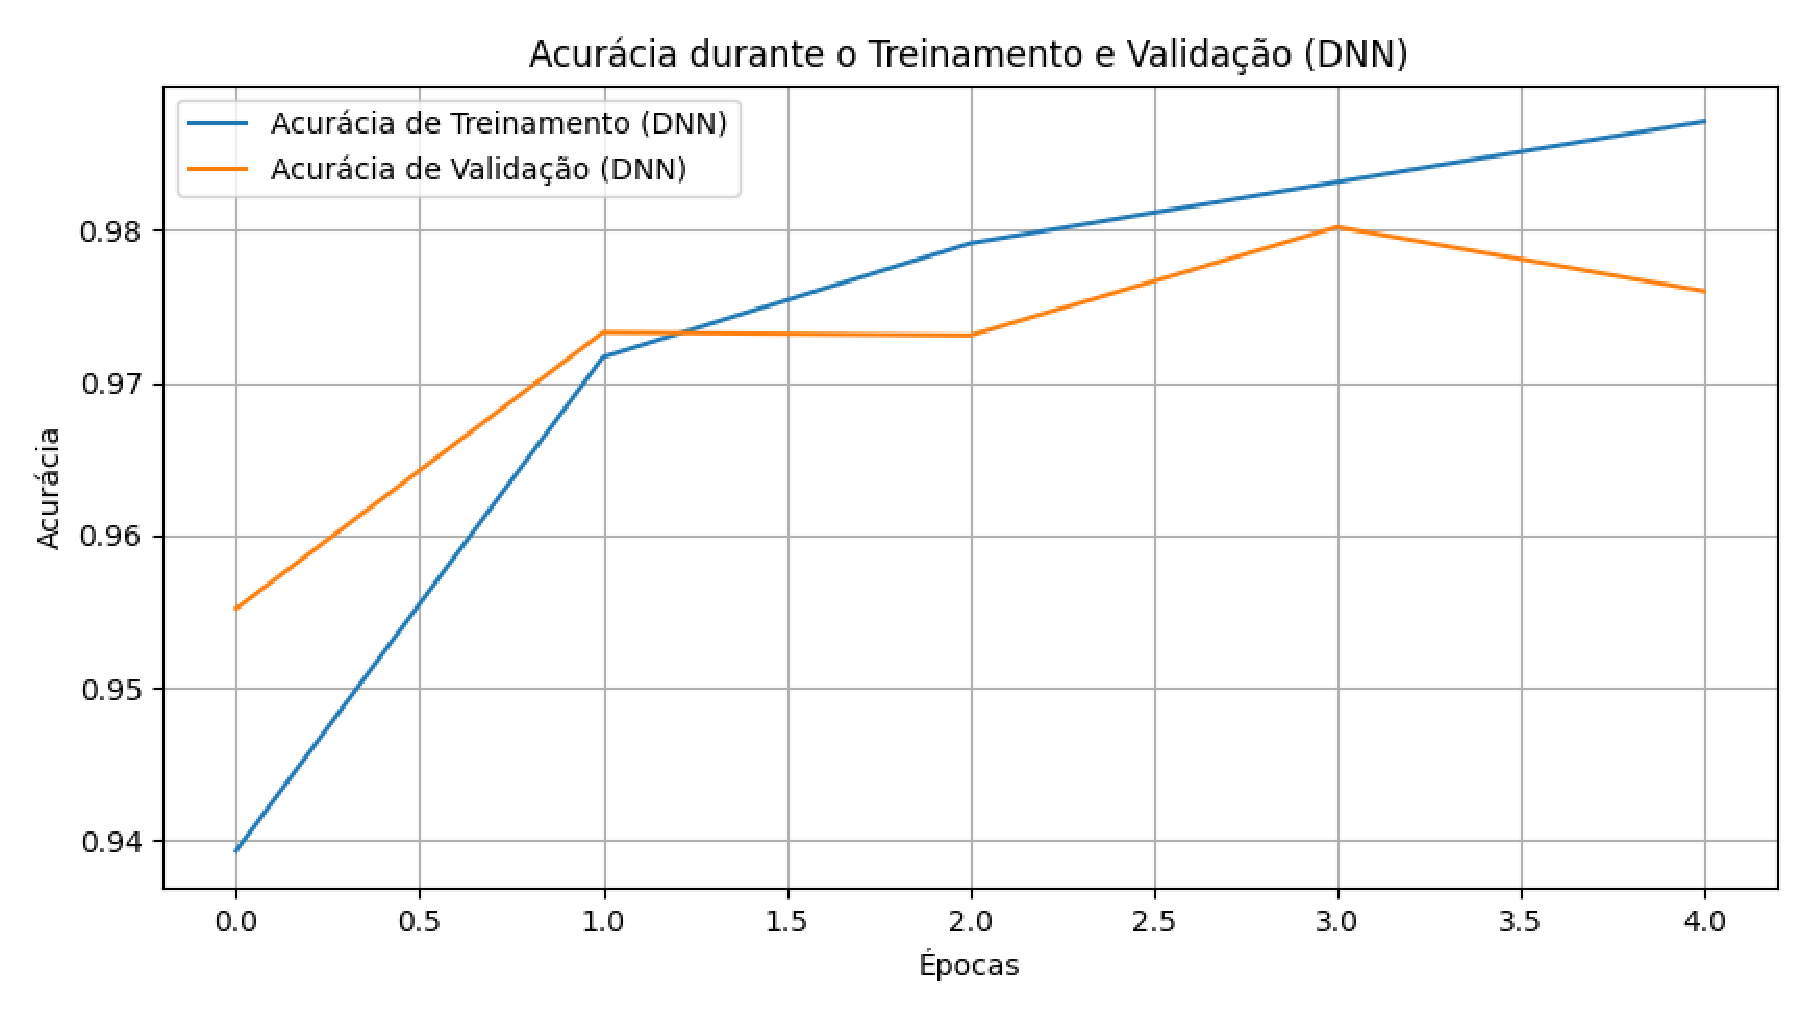
\includegraphics[scale=0.4]{figuras/analiseResultados/acuracyDNN.eps}
    \label{fig:acuracyDNN}
    \fonte{Elaborado pelo autor.}
\end{figure}

Durante o treinamento, que ocorreu ao longo de 50 épocas, observamos uma evolução gradual da acurácia. Na primeira época, o modelo atingiu uma acurácia de 73,94\%, e ao final do treinamento, a acurácia nos dados de teste alcançou 89,69\% (Figura \ref{fig:acuracyDNN}). O modelo demonstrou boa capacidade de generalização para os dados de teste, indicando que foi capaz de captar os padrões das imagens de roupas e calçados presentes na base Fashion-MNIST. A perda de validação também apresentou uma tendência de queda ao longo do treinamento, apesar de ter flutuado um pouco após a 30ª época, sugerindo um leve overfitting que pode ser melhorado com ajustes de hiperparâmetros ou técnicas de regularização mais avançadas, como pode ser observado na Figura \ref{fig:lossDNN}.

\begin{figure}[ht]
    \centering
    \caption{Curvas de perda do modelo centralizado - DNN}
    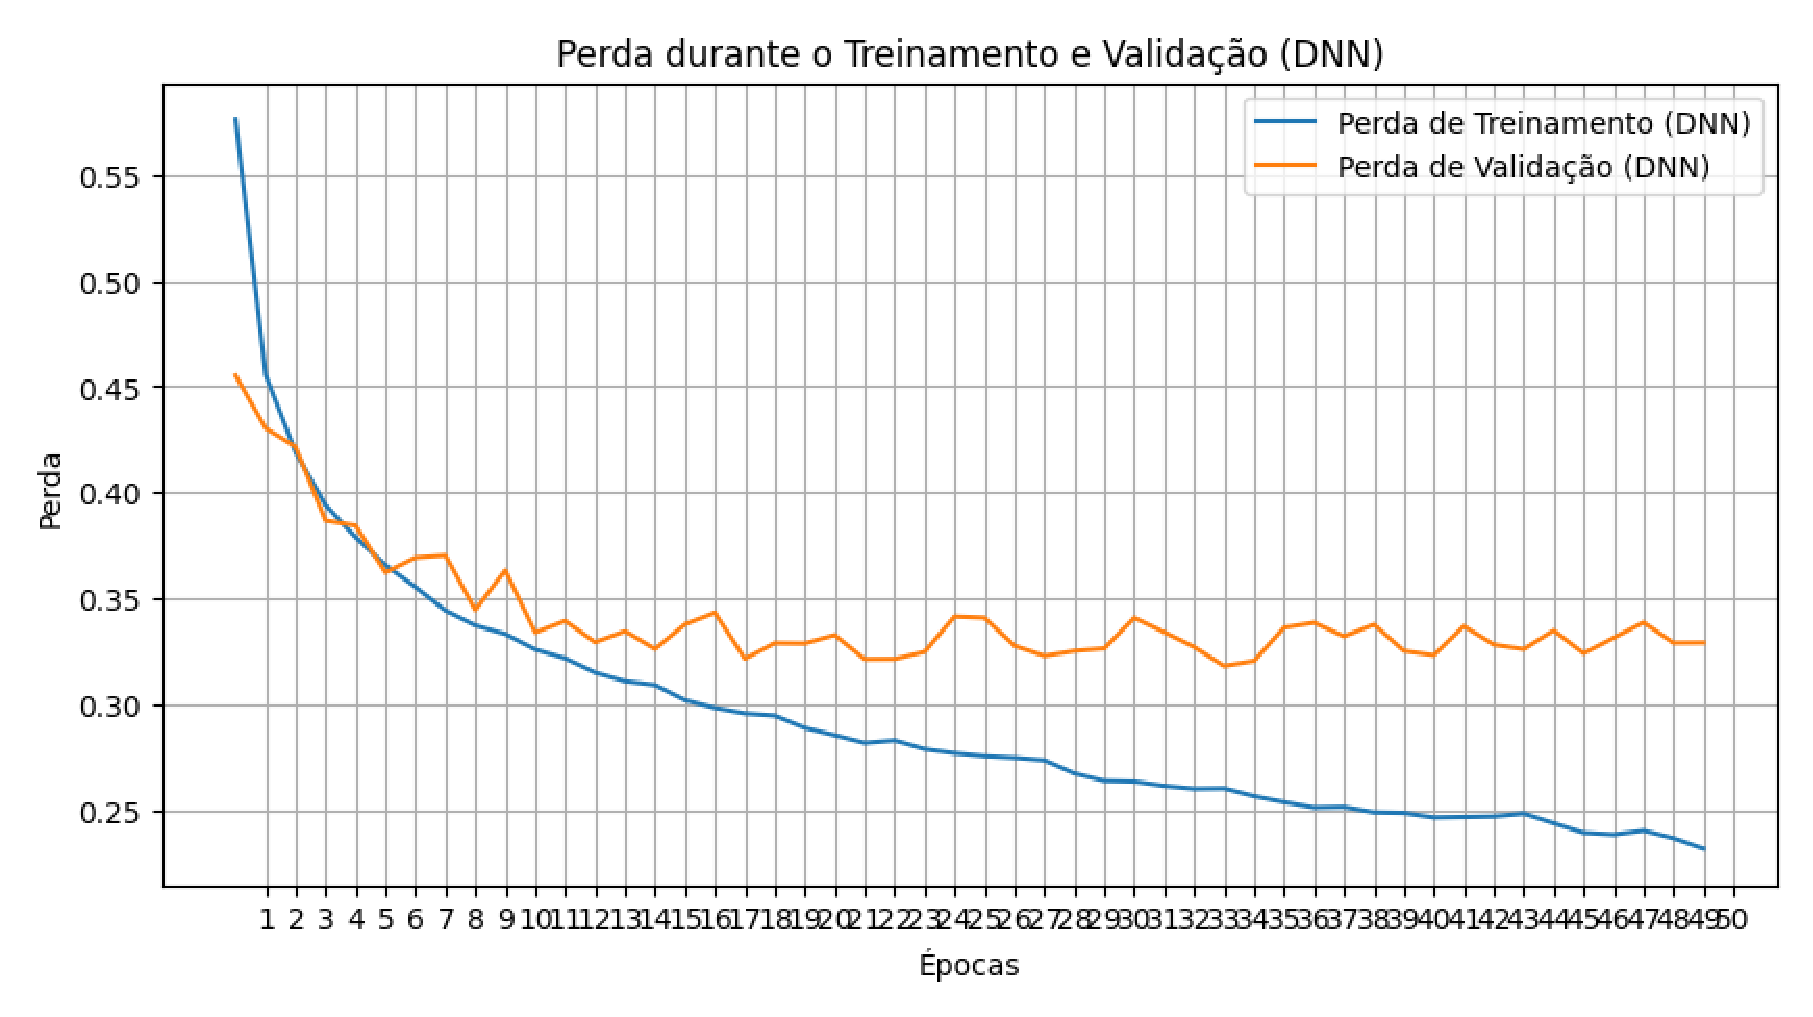
\includegraphics[scale=0.4]{figuras/analiseResultados/lossDNN.eps}
    \label{fig:lossDNN}
    \fonte{Elaborado pelo autor.}
\end{figure}

Em termos de tempo de treinamento, o modelo DNN exigiu aproximadamente 64 minutos (3856 segundos) para ser treinado, o que reflete a complexidade da arquitetura e o tempo necessário para ajustar os parâmetros com uma taxa de aprendizado reduzida para melhorar a convergência. Comparando com os modelos mais simples como o MLP, o DNN obteve um desempenho de acurácia superior, devido à sua maior capacidade de representação e número de parâmetros. No entanto, em termos de tempo, o DNN foi mais lento que os outros modelos centralizados, o que era esperado, dada a profundidade da rede e o número de camadas e neurônios envolvidos.

\section{Resultados do Modelo Federado}

O modelo federado criado para este projeto foi projetado para treinar uma Rede Neural Convolucional (CNN) em um cenário distribuído utilizando dados descentralizados da base Fashion-MNIST. A CNN possui duas camadas convolucionais seguidas de pooling, uma camada totalmente conectada de 128 neurônios e, por fim, uma camada de saída com softmax para as 10 classes do conjunto de dados. A arquitetura foi escolhida para equilibrar a complexidade com o desempenho, enquanto a estratégia federada permitiu o treinamento local em múltiplos clientes sem centralizar os dados. As métricas analisadas incluem acurácia, acurácia top-3 e perda ao longo de 20 rodadas de treinamento.

\subsection{Acurácia por Rodada}

A acurácia categórica medida ao longo das rodadas indica a porcentagem de previsões corretas do modelo considerando apenas a classe mais provável. Na primeira rodada, a acurácia inicial foi de 71,58\%, o que já era uma base sólida considerando o treinamento distribuído e a variedade dos dados em diferentes dispositivos. À medida que o treinamento avançou, a acurácia foi aumentando, chegando a 91,62\% na vigésima rodada. A expectativa era que o modelo federado convergisse para uma acurácia próxima à obtida por um modelo centralizado, mas com desafios como a variabilidade nos dados de diferentes clientes. A acurácia por rodada é apresentada na Figura \ref{fig:acuracyFederated}.

\begin{figure}[ht]
    \centering
    \caption{Curvas de acurácia do modelo federado}
    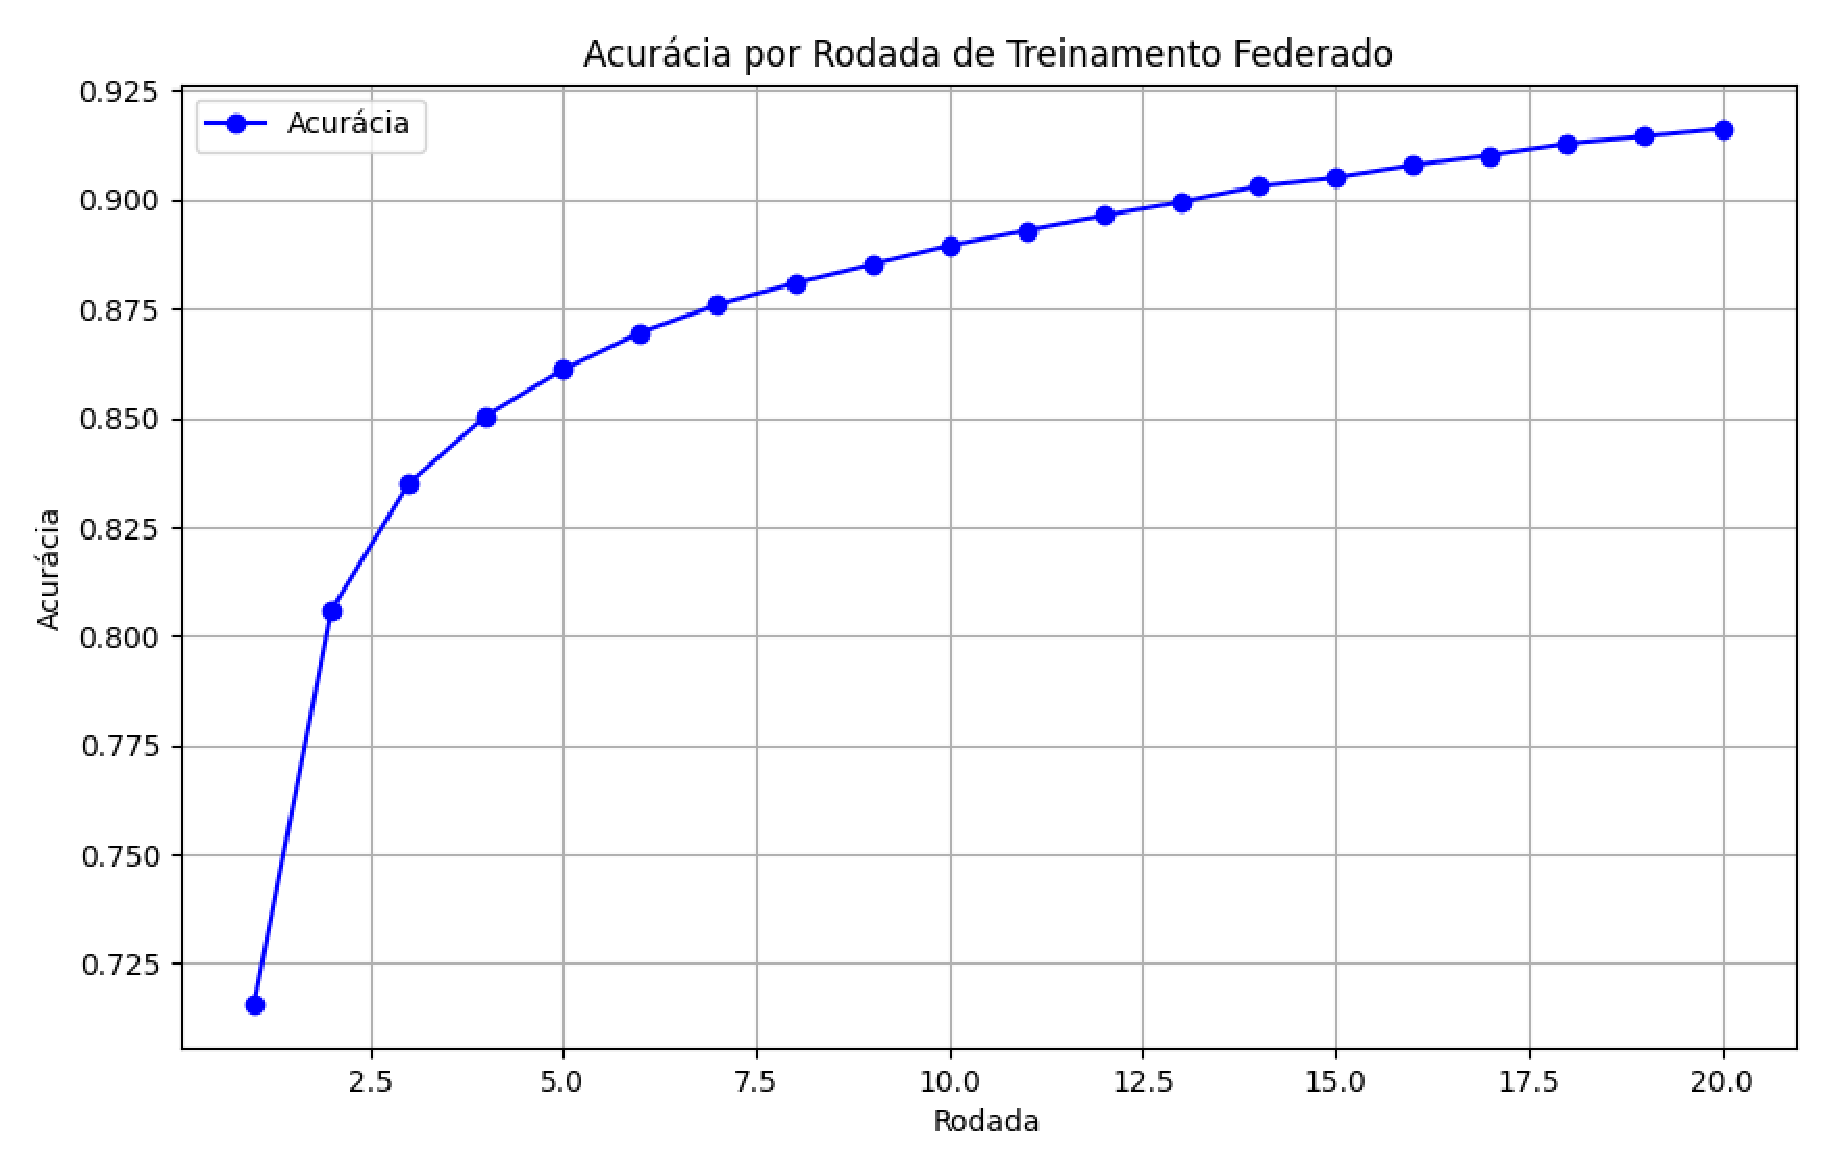
\includegraphics[scale=0.4]{figuras/analiseResultados/acuracyFederated.eps}
    \label{fig:acuracyFederated}
    \fonte{Elaborado pelo autor.}
\end{figure}

A melhoria constante ao longo das rodadas demonstra que, apesar das limitações inerentes ao aprendizado federado, a rede neural conseguiu aprender de maneira eficiente. Entretanto, ajustes finos, como a otimização dos parâmetros e o balanceamento dos dados entre os clientes, poderiam ainda mais aprimorar o desempenho.

\subsection{Acurácia \textit{Top-3}}

A utilização da métrica de acurácia top-3 em um modelo simples, que à primeira vista não parece exigir tal métrica, pode gerar questionamentos. No entanto, há uma justificativa técnica e prática para trazê-la ao contexto de modelos de aprendizado federado, mesmo em cenários menos complexos. A acurácia tradicional, ou top-1, avalia se a previsão feita pelo modelo corresponde exatamente à classe correta. Já a acurácia top-3 expande essa perspectiva, permitindo que a previsão correta seja considerada válida se estiver entre as três principais respostas dadas pelo modelo.

Por que então aplicar a acurácia top-3 em um modelo simples? A resposta está na capacidade dessa métrica de fornecer uma visão mais abrangente da capacidade do modelo em capturar relações próximas entre classes. Quando o modelo lida com dados que possuem classes muito similares entre si – como imagens no conjunto de dados CIFAR-10 ou MNIST – pode ser difícil determinar com precisão se um objeto pertence a uma classe específica, especialmente em casos onde diferentes classes compartilham características visuais ou padrões complexos. Assim, a acurácia top-3 ajuda a revelar se o modelo está, de fato, fazendo previsões significativas, mesmo que a primeira escolha não seja exatamente correta.

Em um cenário real, como em uma aplicação de reconhecimento de imagem em smartphones, o dispositivo pode estar treinando com imagens locais que variam significativamente das imagens em outros dispositivos. A acurácia top-3 se torna útil aqui porque permite observar se o modelo está, ao menos, identificando as classes mais próximas de forma coerente, mesmo que em alguns casos não acerte exatamente a classe correta no top-1. Isso é especialmente importante quando há variações nos dados ou ruído nas entradas.

A acurácia top-3 reflete a capacidade do modelo de incluir a classe correta entre as três principais previsões feitas. Esta métrica é particularmente útil em cenários onde a classificação pode ter ambiguidade e uma das classes mais prováveis pode ser a correta. No modelo federado, a acurácia top-3 começou em 93,95\% e subiu para 99,50\% na rodada final. A acurácia top-3 é apresentada na Figura \ref{fig:acuracyTop3Federated}.

\begin{figure}[ht]
    \centering
    \caption{Curvas de acurácia \textit{Top-3} do modelo federado}
    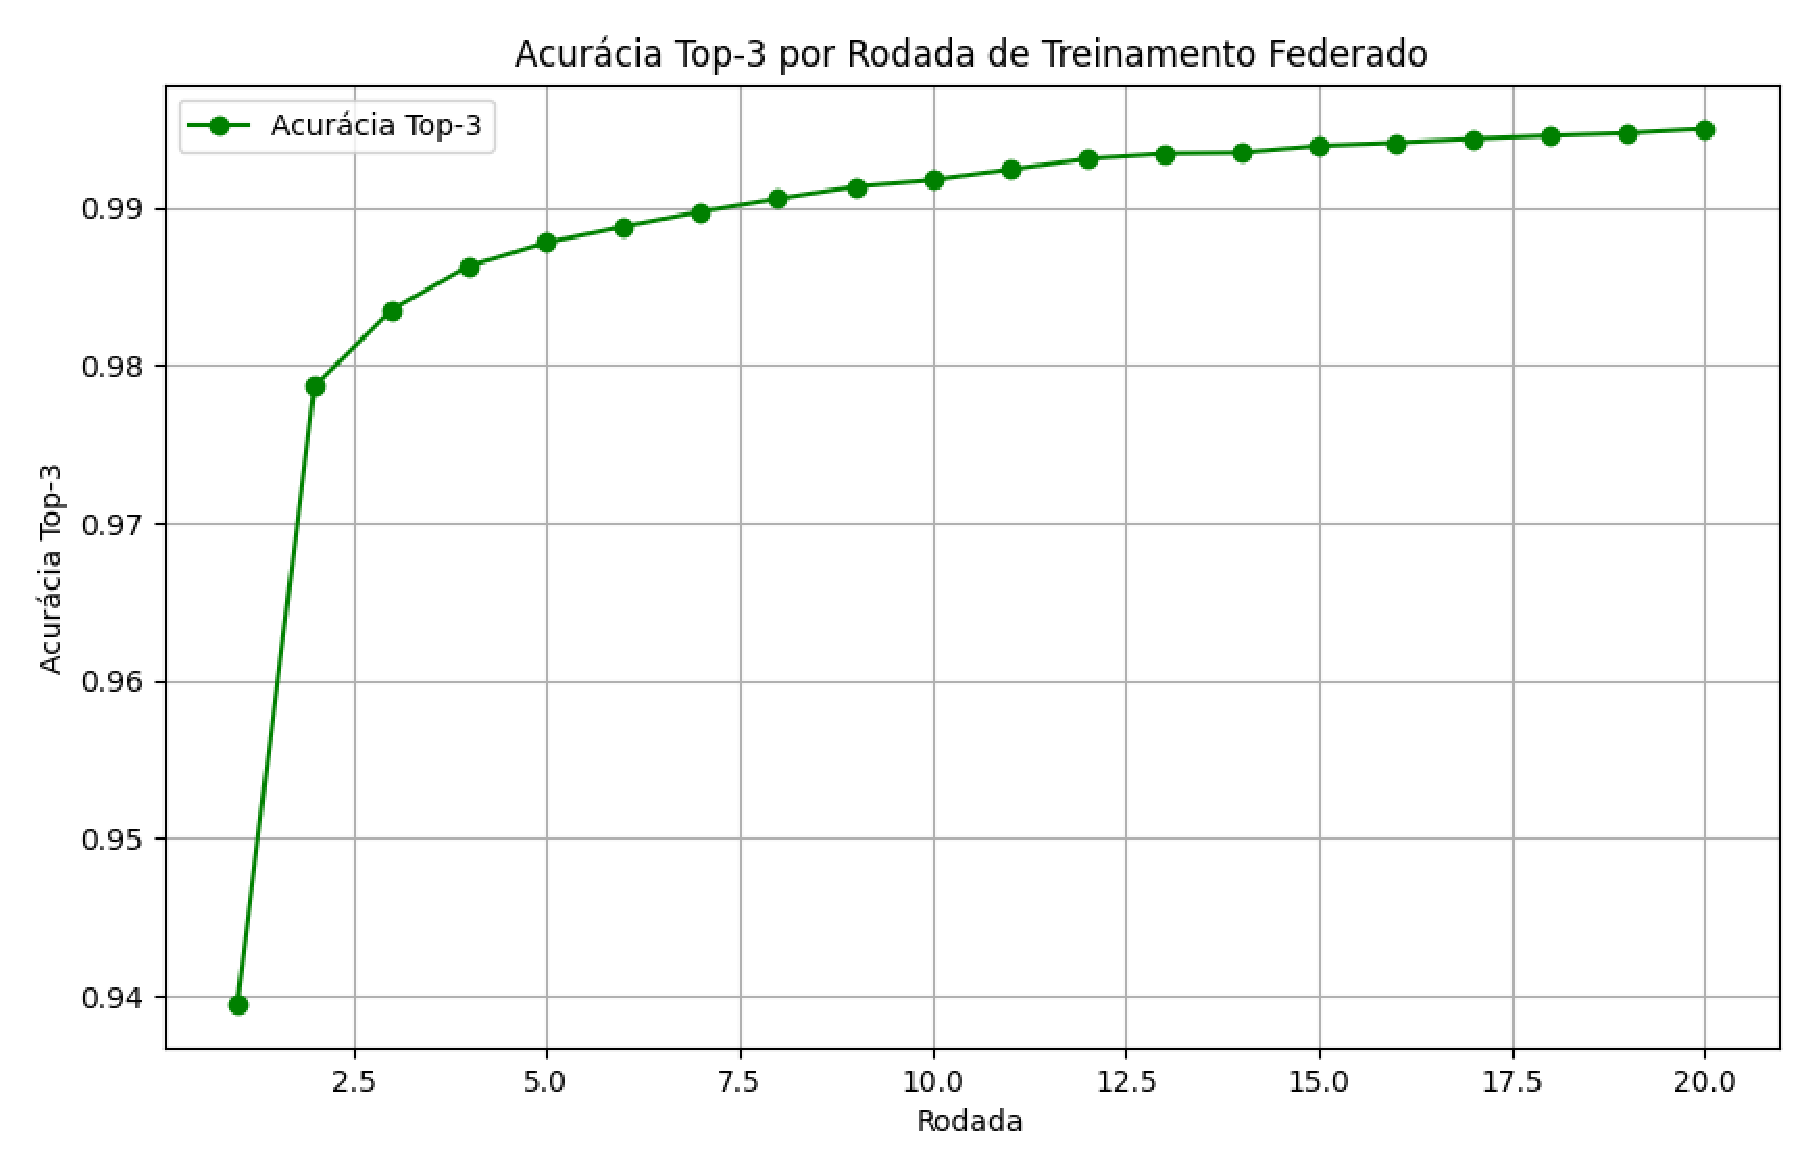
\includegraphics[scale=0.4]{figuras/analiseResultados/acuracyTop3Federated.eps}
    \label{fig:acuracyTop3Federated}
    \fonte{Elaborado pelo autor.}
\end{figure}

Esse resultado sugere que o modelo federado pode ser particularmente eficaz em cenários onde a precisão absoluta de top-1 pode não ser suficiente, como em recomendações de produtos ou sistemas de detecção com baixa margem de erro.

\subsection{Perda por Rodada}

A perda foi monitorada como uma métrica que quantifica o erro do modelo, sendo uma medida crítica durante o processo de otimização. Na primeira rodada, a perda era relativamente alta, com um valor de 0,773, o que reflete a incerteza inicial do modelo ao fazer previsões em um cenário federado. Ao longo do treinamento, houve uma queda consistente na perda, que foi reduzida para 0,227 ao final da vigésima rodada. A perda por rodada é apresentada na Figura \ref{fig:lossFederated}.

\begin{figure}[ht]
    \centering
    \caption{Curvas de perda do modelo federado}
    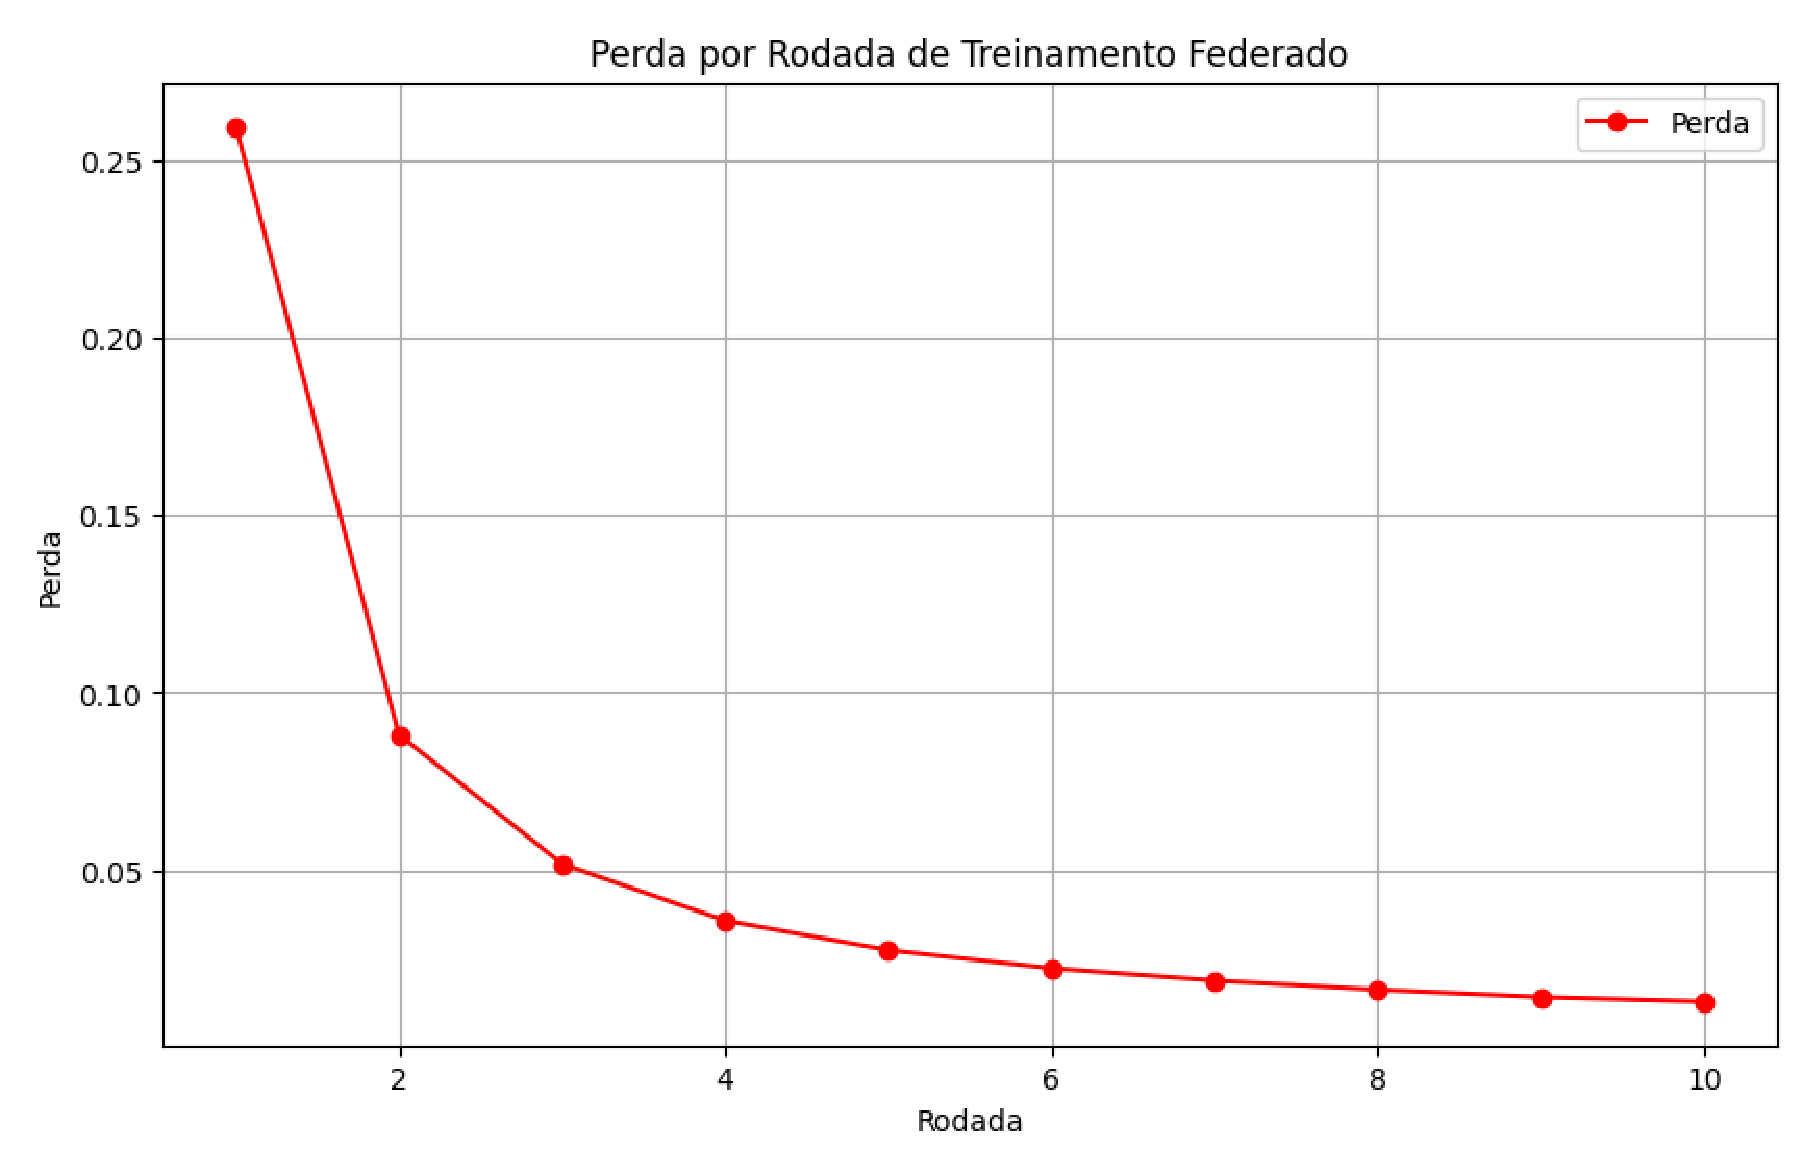
\includegraphics[scale=0.4]{figuras/analiseResultados/lossFederated.eps}
    \label{fig:lossFederated}
    \fonte{Elaborado pelo autor.}
\end{figure}

A expectativa era de que a perda diminuísse à medida que o modelo ajustasse seus pesos com base nas atualizações federadas, embora a velocidade da convergência possa ser impactada pela comunicação entre os dispositivos e a distribuição não homogênea dos dados. A redução da perda confirma que o modelo aprendeu de maneira estável ao longo das rodadas, e, embora o treinamento federado tenha suas complexidades, ele foi capaz de atingir um desempenho competitivo com modelos centralizados.

\section{Desempenho entre os Modelos}

Nesta seção, analisamos o desempenho dos modelos centralizados e federados aplicados ao conjunto de dados Fashion-MNIST. As métricas de avaliação utilizadas incluem acurácia, acurácia \textit{Top-3} e perda. A comparação entre o modelo de aprendizado federado e os modelos centralizados oferece insights valiosos sobre a eficácia e a eficiência das diferentes abordagens.

\subsection{Acurácia}

A acurácia é a principal métrica usada para avaliar a proporção de previsões corretas feitas pelo modelo em relação ao total de previsões. Nos modelos centralizados desenvolvidos com diferentes técnicas de treinamento (CNN, MLP, DNN), a acurácia foi consistentemente alta, com a CNN alcançando uma acurácia de 91,4\% após 50 épocas de treinamento, o MLP atingindo 89,0\%, e o DNN registrando 89,6\%. Esses números refletem um desempenho sólido, especialmente considerando o uso de um conjunto de dados como o Fashion-MNIST. O modelo federado, por outro lado, apresentou uma acurácia final de 91,6\% após 20 rodadas de treinamento, o que está alinhado com as expectativas de desempenho. A comparação da acurácia dos modelos Centralizados e Federado é apresentada na Figura \ref{fig:acuracyComparison}.

\begin{figure}[ht]
    \centering
    \caption{Comparação de acurácia entre os modelos centralizados e federados}
    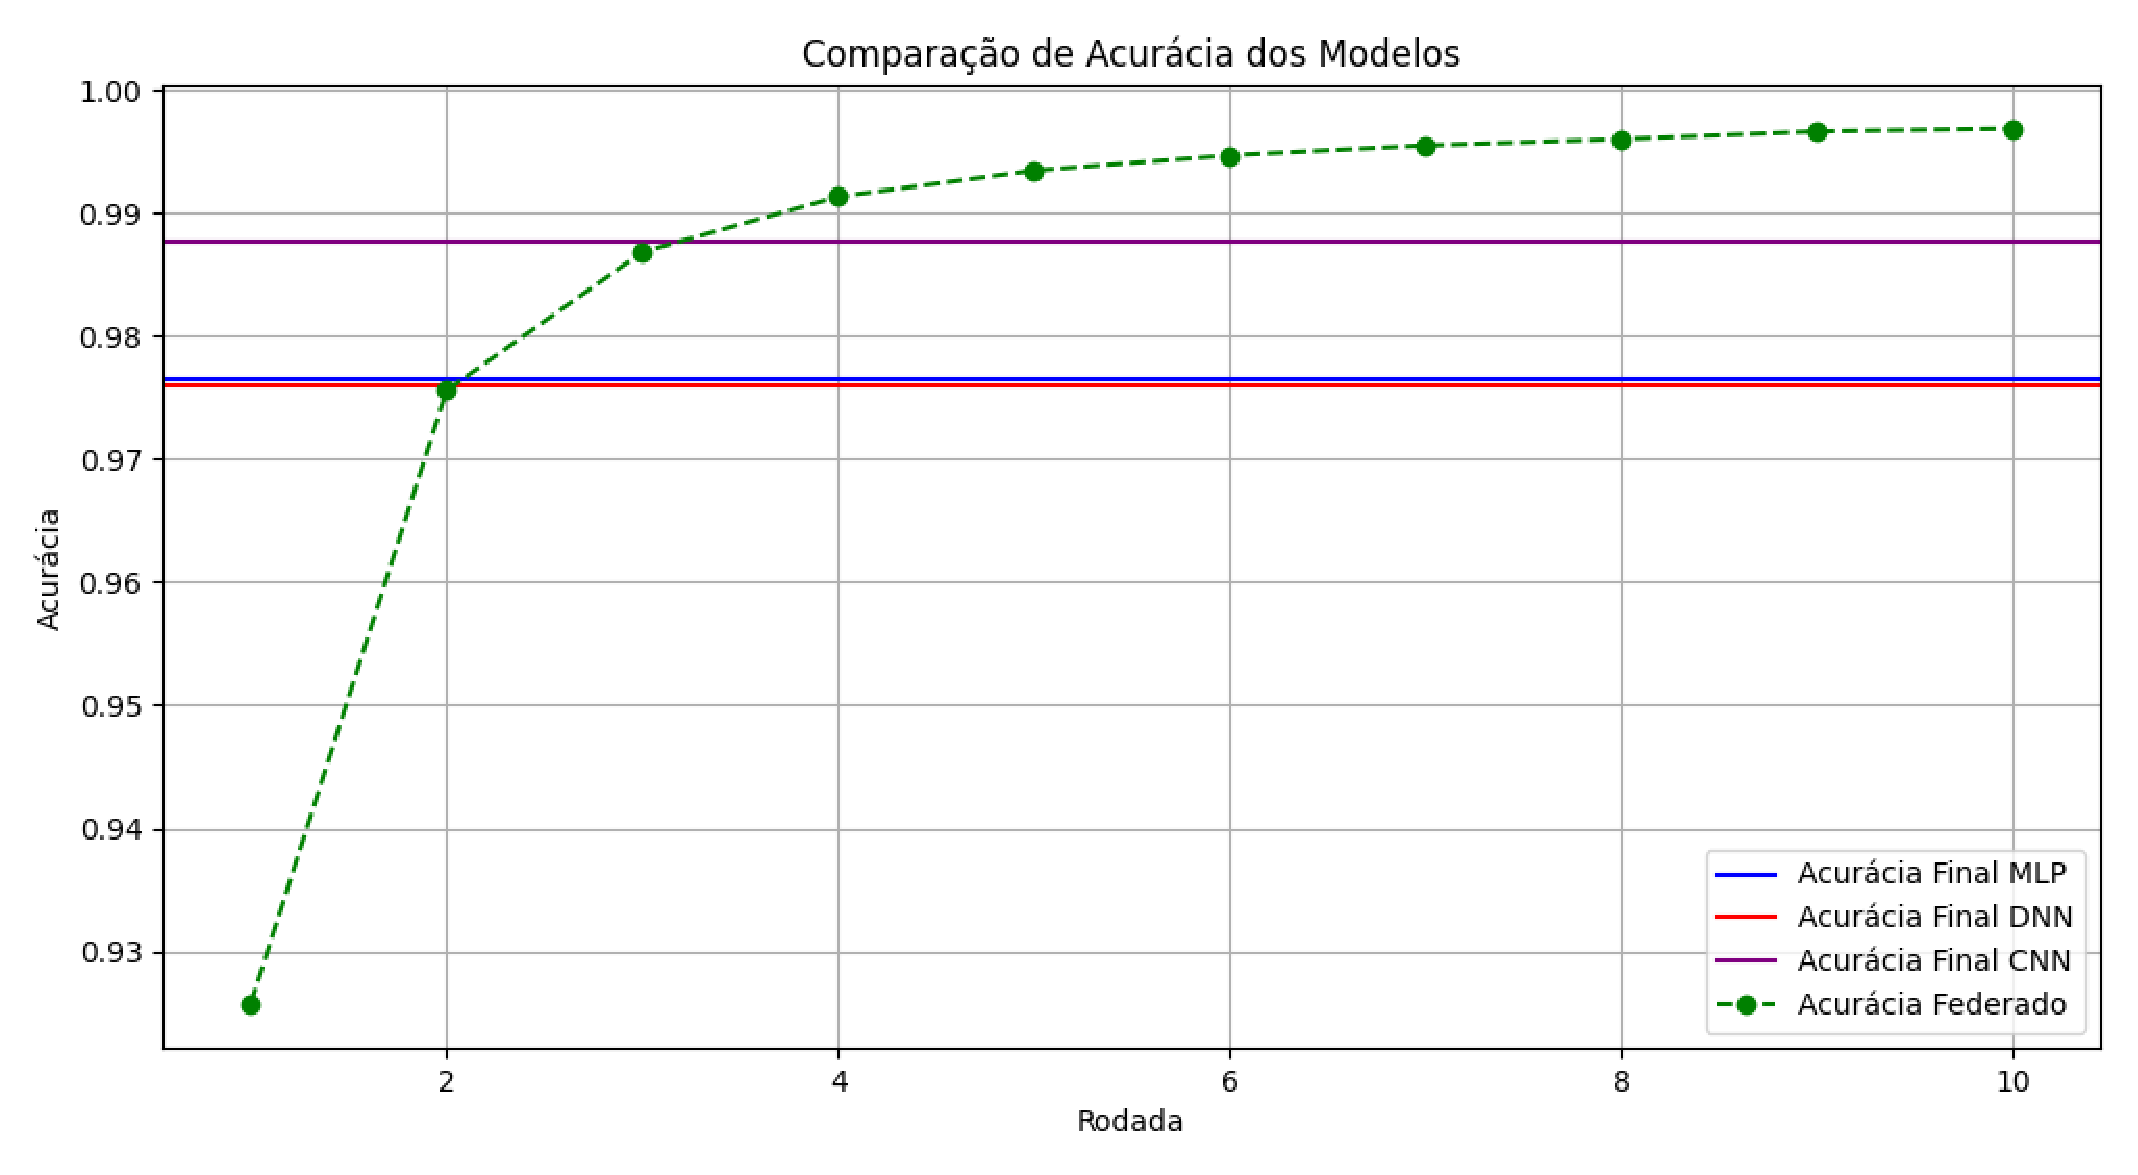
\includegraphics[scale=0.4]{figuras/analiseResultados/acuracyComparison.eps}
    \label{fig:acuracyComparison}
    \fonte{Elaborado pelo autor.}
\end{figure}

Esperava-se que o modelo federado atingisse níveis comparáveis aos modelos centralizados, apesar das limitações inerentes à descentralização dos dados e à variação entre os dispositivos. De maneira geral, a acurácia do modelo federado mostrou-se competitiva, evidenciando que a abordagem distribuída pode ser eficaz em cenários reais sem sacrificar significativamente a precisão.

\subsection{Perda}

A perda é uma métrica que reflete o erro acumulado do modelo ao longo do treinamento. Em modelos de classificação como os utilizados neste estudo, a perda é geralmente expressa através da função de erro de entropia cruzada. Para os modelos centralizados, a perda final foi de 0,48 para a CNN, 0,31 para o MLP e 0,33 para o DNN, indicando que o erro foi bem minimizado ao longo do processo de treinamento. O modelo federado, por sua vez, apresentou uma perda de 0,23 na última rodada, sugerindo que ele foi capaz de reduzir o erro de maneira eficiente, mesmo em um cenário onde os dados estão distribuídos e não centralizados. Como pode ser observado na Figura \ref{fig:lossComparison}.

\begin{figure}[ht]
    \centering
    \caption{Comparação de perda entre os modelos centralizados e federados}
    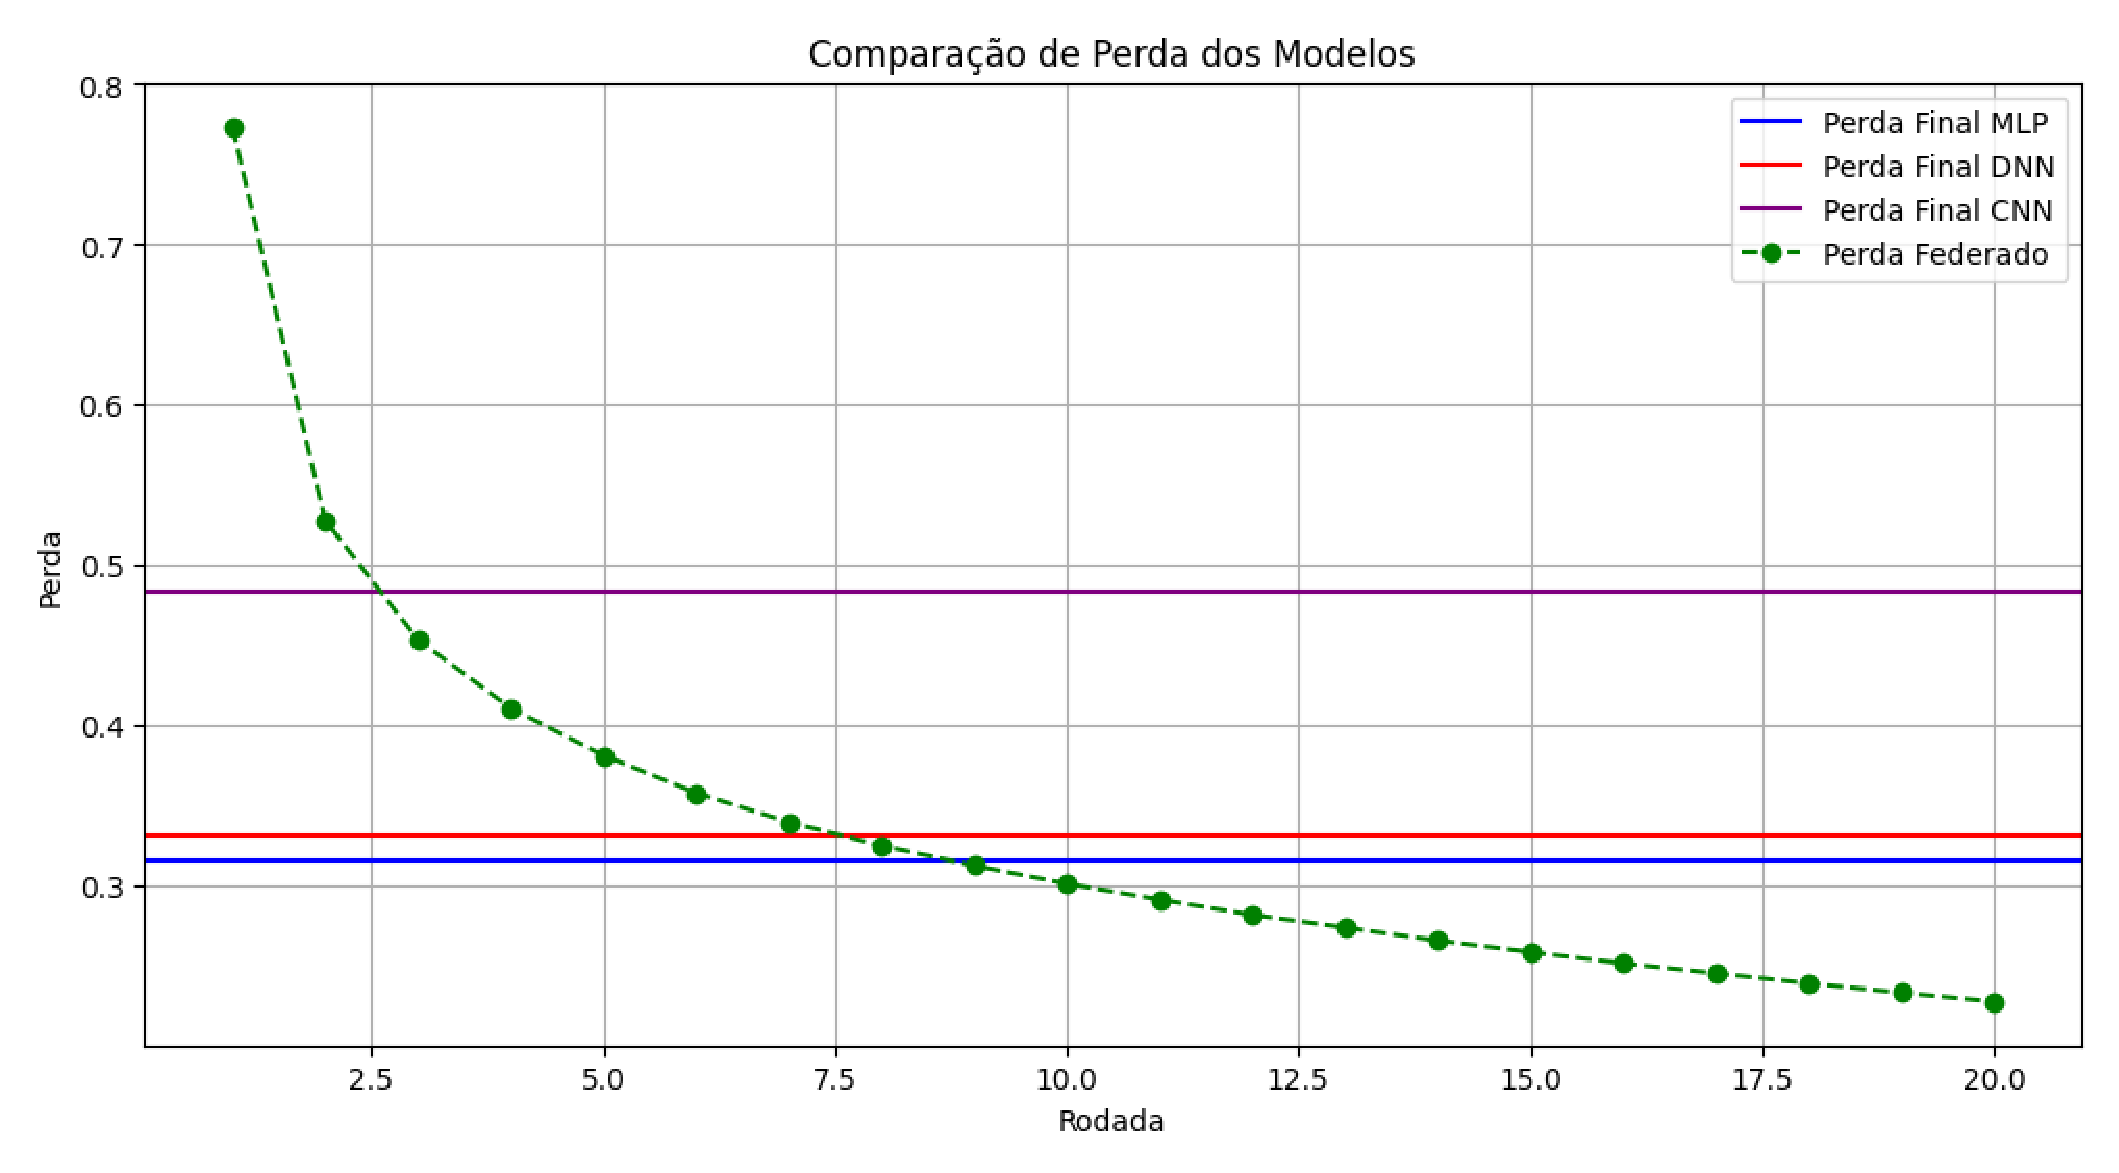
\includegraphics[scale=0.4]{figuras/analiseResultados/lossComparison.eps}
    \label{fig:lossComparison}
    \fonte{Elaborado pelo autor.}
\end{figure}

Antes do treinamento, a expectativa era de que a perda no modelo federado fosse ligeiramente maior do que nos modelos centralizados, devido à complexidade adicional introduzida pela comunicação entre dispositivos e pelas diferenças nos dados locais. No entanto, o resultado final foi positivo, com a perda do modelo federado sendo inferior em algumas rodadas, o que indica que o processo federado conseguiu aprender de forma eficiente, mesmo com as restrições do ambiente distribuído.

\subsection{Acurácia \textit{Top-3}}

A acurácia top-3 mede a capacidade do modelo de prever a classe correta dentro das três classes mais prováveis, o que é especialmente útil em cenários onde há ambiguidades entre classes. Para os modelos centralizados, essa métrica não foi usada inicialmente, mas foi incluída no modelo federado como uma forma de explorar cenários mais realistas de classificação. A acurácia top-3 do modelo federado atingiu 99,5\% na última rodada, o que significa que, mesmo em casos onde o modelo não acertou a classe exata, ele foi capaz de incluir a resposta correta entre suas três principais previsões na maioria das vezes.

Isso era esperado, uma vez que a acurácia top-3 geralmente tende a ser mais alta do que a acurácia categórica, dado que o modelo tem mais chances de acertar dentro de um intervalo maior de possibilidades.  A alta acurácia top-3 no modelo federado sugere que ele poderia ser altamente eficaz em cenários de produção, onde a precisão absoluta nem sempre é o critério mais importante.

\section{Considerações Finais}

Comparando o desempenho geral dos modelos, pode-se observar que o modelo federado apresentou desempenho semelhante, e em alguns casos, até superior em relação aos modelos centralizados em termos de acurácia e perda. A principal vantagem do aprendizado federado é a preservação da privacidade dos dados, mas isso geralmente vem com o custo de maior complexidade no treinamento e maiores exigências computacionais. No entanto, os resultados demonstram que, com as devidas otimizações, o aprendizado federado pode atingir níveis de desempenho muito próximos dos modelos tradicionais centralizados, sem comprometer significativamente a precisão ou aumentar excessivamente a perda. A inclusão da acurácia top-3 também destaca o potencial do aprendizado federado para ser utilizado em cenários de classificação mais complexos, onde várias respostas podem ser válidas.

Em termos de expectativas, esperava-se que os modelos centralizados se saíssem um pouco melhor em acurácia e perda, devido à sua simplicidade e eficiência computacional, mas os resultados mostraram que o modelo federado foi capaz de se manter competitivo. Essa conclusão reforça a ideia de que o aprendizado federado é uma solução viável para cenários descentralizados, onde a privacidade é uma preocupação central, sem sacrificar o desempenho.

\section{Dificuldades e Limitações}

A seção de dificuldades e limitações explora os desafios enfrentados durante o desenvolvimento dos modelos de aprendizado centralizado e federado, as influências dessas dificuldades na escolha da base de dados e as implicações do uso do Google Colab no treinamento dos modelos. Esta análise fornece uma visão crítica sobre as limitações dos métodos de treinamento e os aspectos técnicos que impactaram o progresso e os resultados do projeto.

\subsection{Dificuldades no Desenvolvimento dos Modelos}

Desenvolver modelos de aprendizado centralizado e federado envolveu uma série de desafios técnicos e conceituais. Para os modelos centralizados, como o MLP e o DNN, uma das principais dificuldades foi o ajuste dos hiperparâmetros, como a taxa de aprendizado e o número de camadas e neurônios. A escolha inadequada desses parâmetros pode levar a problemas como overfitting ou underfitting, impactando negativamente a precisão e a capacidade de generalização dos modelos. Além disso, a gestão do treinamento e a monitorização das métricas de desempenho foram essenciais para garantir que o modelo estivesse aprendendo de forma eficaz e não estivesse simplesmente decorando os dados de treinamento.

\subsection{Influência na Escolha da Base de Dados}

A escolha da base de dados Fashion-MNIST foi feita de forma estratégica, levando em consideração a necessidade de um dataset que representasse um cenário de classificação realista, mas que ainda fosse manejável em termos computacionais. Fashion-MNIST apresenta um desafio maior do que o MNIST tradicional, mas ainda assim é uma base de dados controlada e de tamanho razoável, o que facilitou a comparação de resultados entre os diferentes modelos. No entanto, apesar da simplicidade relativa dos dados, a diversidade das imagens de vestuário e as pequenas diferenças entre classes exigiram que os modelos fossem cuidadosamente ajustados para maximizar a precisão sem sobrecarregar os recursos computacionais disponíveis.

\subsection{Impacto do Google Colab no Treinamento dos Modelos}

O uso do Google Colab teve um impacto no desenvolvimento e no treinamento dos modelos. Google Colab fornece uma plataforma acessível e com recursos computacionais relativamente poderosos, como GPUs, o que facilitou o treinamento dos modelos, especialmente para o modelo DNN que exige maior capacidade computacional. No entanto, existem limitações associadas ao uso de Google Colab, como restrições de tempo de execução e limitações de memória. Essas restrições podem impactar o treinamento de modelos mais complexos ou o uso de grandes conjuntos de dados.

\subsection{Limitações dos Métodos de Treinamento}

Os métodos de treinamento centralizado e federado apresentam suas próprias limitações. No treinamento centralizado, um desafio é a necessidade de grandes volumes de dados e poder computacional para alcançar resultados precisos e generalizáveis. Modelos mais complexos podem exigir ajustes finos e otimização que podem não ser práticos em todas as situações. Além disso, o treinamento centralizado não aborda diretamente a questão da privacidade dos dados, o que pode ser uma limitação significativa em contextos onde a proteção da privacidade é essencial.

Por outro lado, o aprendizado federado, embora ofereça vantagens significativas em termos de privacidade e segurança dos dados, enfrenta limitações relacionadas à comunicação e sincronização entre os clientes. A agregação de modelos locais pode ser influenciada pela heterogeneidade dos dados e pelas condições variáveis de treinamento nos diferentes clientes. Além disso, o custo computacional e a complexidade do protocolo de treinamento federado podem ser desafiadores, especialmente quando se lida com um grande número de clientes e uma vasta quantidade de dados.